% !TEX encoding = UTF-8
% !TEX program = xelatex
\documentclass[12pt,a4paper]{article}
\usepackage[paperwidth=210mm, paperheight=297mm, left=0.75in, right=0.75in, bottom=1in, top=1in]{geometry}
\usepackage{polyglossia}
\setdefaultlanguage[babelshorthands]{italian}
\usepackage{fontspec}
\usepackage{graphicx}
\usepackage{blindtext}
\usepackage{wrapfig}

\frenchspacing
\makeindex

\begin{document}
\title{\vspace{-70pt}NOME}
\author{AUTORE}
\date{}
\maketitle
\pagestyle{empty}
\thispagestyle{empty}

\begin{wrapfigure}{r}{0.35\textwidth}
  \vspace{-10pt}
  \begin{center}
    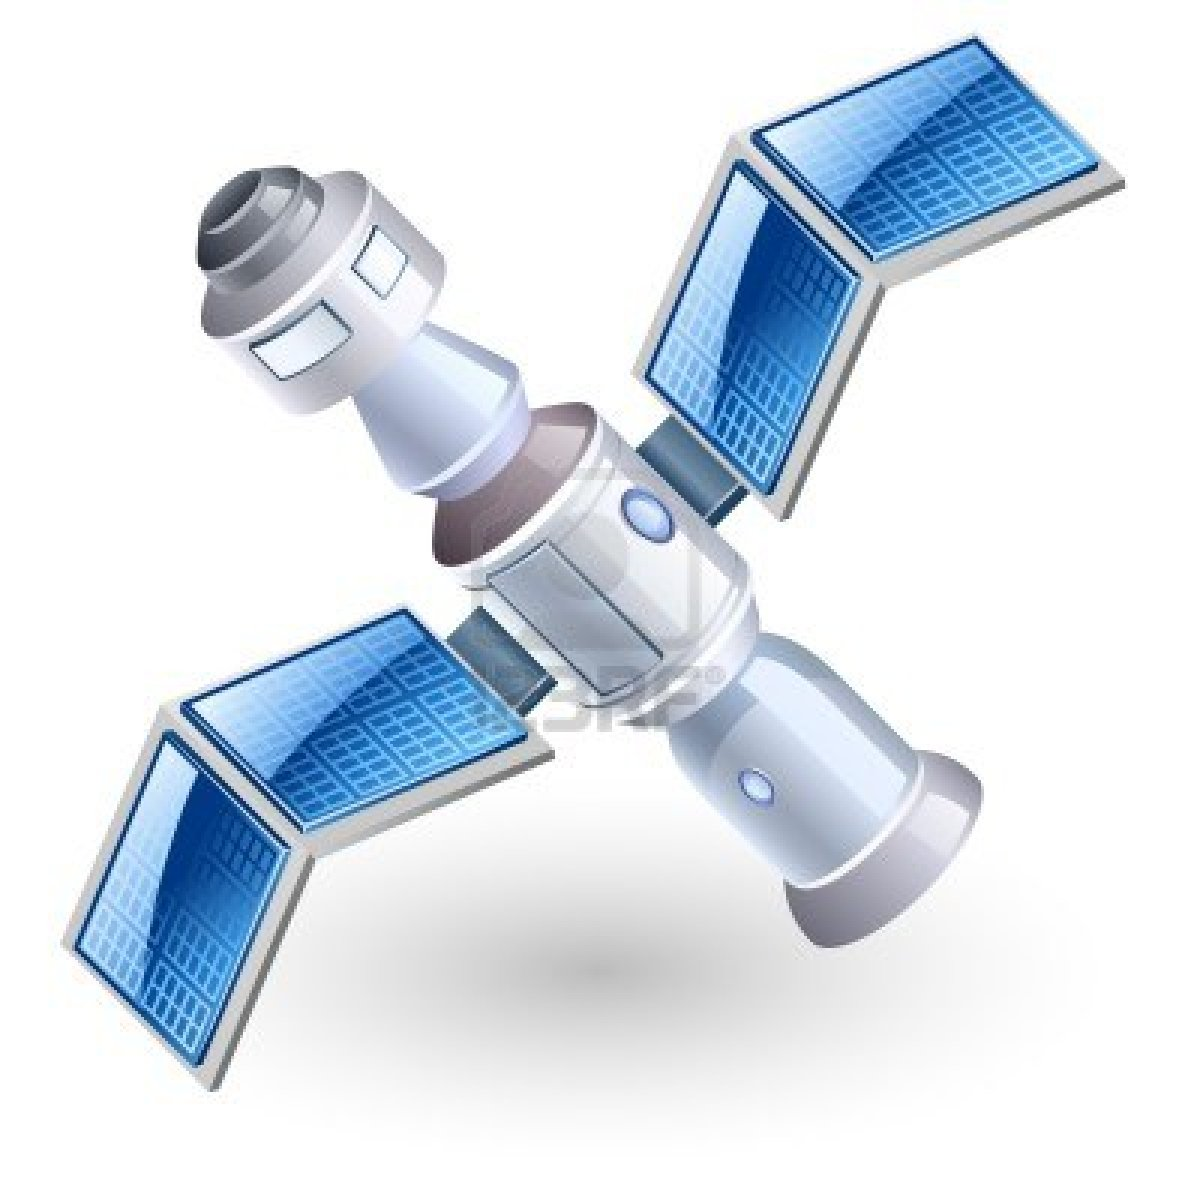
\includegraphics[width=0.30\textwidth]{satellite}
  \end{center}
  \vspace{-20pt}
\end{wrapfigure}

% aggiungere asterischi
% cambiare nome e autore
% spostare figura
% pack

\end{document}